\documentclass[11pt,a4paper]{article}
\usepackage[utf8]{inputenc}
\usepackage[spanish]{babel}
\usepackage{geometry}
\geometry{a4paper, margin=1in, headheight=14pt}
\usepackage{graphicx}
\usepackage{xcolor}
\usepackage{hyperref}
\usepackage{booktabs}
\usepackage{fancyhdr}
\usepackage{titlesec}
\usepackage{listings}
\usepackage{amsmath}
\usepackage{tcolorbox}
\usepackage{enumitem}
\usepackage{float}

% --- Definición de Colores de la Marca SmartSaver ---
\definecolor{primaryblue}{HTML}{3B82F6}
\definecolor{secgreen}{HTML}{10B981}
\definecolor{warnorange}{HTML}{F59E0B}
\definecolor{critred}{HTML}{EF4444}
\definecolor{darkslate}{HTML}{0F172A}
\definecolor{lightbg}{HTML}{F8FAFC}
\definecolor{bordergray}{HTML}{E2E8F0}

% --- Configuración de Hipervínculos ---
\hypersetup{
    colorlinks=true,
    linkcolor=primaryblue,
    filecolor=secgreen,      
    urlcolor=primaryblue,
    pdftitle={Manual de Usuario - SmartSaver},
    pdfpagemode=FullScreen,
}

% --- Estilo de Página y Encabezados ---
\pagestyle{fancy}
\fancyhf{}
\fancyhead[L]{\textcolor{darkslate}{\textbf{SmartSaver} --- Manual de Usuario}}
\fancyhead[R]{\textcolor{darkslate}{IoT Mini-UPS Control}}
\fancyfoot[C]{\thepage}
\renewcommand{\headrulewidth}{0.5pt}
\renewcommand{\footrulewidth}{0.5pt}

% --- Formato de Secciones ---
\titleformat{\section}
  {\color{primaryblue}\normalfont\Large\bfseries}
  {\thesection}{1em}{}
\titleformat{\subsection}
  {\color{darkslate}\normalfont\large\bfseries}
  {\thesubsection}{1em}{}

% --- Cajas Personalizadas de Información ---
\newtcolorbox{infoBox}{
  colback=lightbg,
  colframe=primaryblue,
  fonttitle=\bfseries,
  coltitle=white,
  title=Información Importante,
  arc=5pt
}

\newtcolorbox{alertBox}{
  colback=lightbg,
  colframe=critred,
  fonttitle=\bfseries,
  coltitle=white,
  title=Alerta de Seguridad,
  arc=5pt
}

\begin{document}
\pagenumbering{roman}

% ==========================================
% PORTADA
% ==========================================
\begin{titlepage}
    \centering
    \vspace*{2cm}
    {\Huge \bfseries \color{primaryblue} SMARTSAVER} \\[0.4cm]
    {\Large \bfseries \color{darkslate} Sistema de Monitoreo y Control Móvil para Dispositivos Smart Mini-UPS} \\[1.5cm]
    \vspace*{0.5cm}
    \begin{tcolorbox}[colback=primaryblue, colframe=primaryblue, width=4cm, height=4cm, arc=15pt, boxrule=0pt, colupper=white, valign=center, halign=center]
        \centering
        \vspace*{0.5cm}
        {\Huge \bfseries S} \\[0.1cm]
        {\small \bfseries SMART\kern-0.05em SAVER}
    \end{tcolorbox}
    \vspace*{1.5cm}
    
    {\large \textbf{Manual de Usuario Oficial}} \\[0.5cm]
    {\large Versión 5.1} \\[2cm]
    
    \textbf{Desarrollado para:} \\
    Monitoreo de Nodos Inteligentes IoT basados en ESP32 \\[1cm]
    
    \vfill
    {\large \today}
\end{titlepage}

\newpage
\tableofcontents
\newpage
\pagenumbering{arabic}

% ==========================================
% SECCIÓN 1: INTRODUCCIÓN
% ==========================================
\section{Introducción y Descripción General}
El sistema \textbf{SmartSaver} es una solución tecnológica integral diseñada para optimizar y controlar sistemas de alimentación ininterrumpida inteligente (\textit{Smart Mini-UPS}) basados en microcontroladores ESP32. Su principal objetivo es proporcionar a los usuarios una interfaz móvil moderna, intuitiva y fluida para monitorear el consumo de energía en tiempo real, programar horarios de uso y configurar límites estrictos de seguridad para prevenir daños en hardware crítico.

\subsection{Arquitectura del Ecosistema}
El ecosistema SmartSaver está compuesto por tres capas principales:
\begin{enumerate}
    \item \textbf{Hardware Smart Mini-UPS (ESP32):} Mide constantemente los valores eléctricos de voltaje (V), corriente (A) y potencia activa (W), ejecutando órdenes locales e informando su telemetría mediante el protocolo MQTT.
    \item \textbf{Servidor Backend (FastAPI, MariaDB y MQTT Broker):} Actúa como base de datos histórica y pasarela de comandos en tiempo real.
    \item \textbf{Aplicación Móvil (React Native, Expo):} Interfaz gráfica (en español) desde la cual el usuario realiza configuraciones avanzadas, visualiza analíticas históricas y gestiona las prioridades de corte de energía.
\end{enumerate}

\begin{infoBox}
Este manual detalla todas las funcionalidades del aplicativo móvil de SmartSaver, guiándolo paso a paso desde el inicio de sesión hasta la exportación de reportes avanzados de consumo.
\end{infoBox}

% ==========================================
% SECCIÓN 2: INICIO DE SESIÓN
% ==========================================
\section{Autenticación e Inicio de Sesión}
Para garantizar la integridad y seguridad de la red de dispositivos, SmartSaver utiliza un protocolo de autenticación robusto basado en \textbf{OAuth 2.1 + OIDC} a través de la plataforma \textbf{Auth0} utilizando el flujo criptográfico \textbf{PKCE (Proof Key for Code Exchange)}.

\subsection{Pasos para el Acceso}
\begin{enumerate}
    \item Al abrir el aplicativo por primera vez, el sistema verificaría las credenciales guardadas en el almacenamiento seguro de su dispositivo (\textit{SecureStore}).
    \item Si no existe una sesión activa o el token de acceso ha expirado sin posibilidad de refresco automático, el sistema mostrará la pantalla de \textbf{Acceso Seguro}.
    \item Presione el botón \textbf{"Iniciar Sesión"}.
    \item Se abrirá un navegador seguro embebido. Ingrese su correo electrónico y contraseña registrados, o utilice proveedores federados (si están disponibles).
    \item Tras autenticarse correctamente, el sistema guardará de forma encriptada sus credenciales y lo redirigirá al \textbf{Dashboard (Panel de Inicio)} de la aplicación.
\end{enumerate}

\subsection{Configuración Inicial del Perfil (Onboarding)}
Una vez que el usuario se autentica por primera vez, el sistema redirige de forma obligatoria a la pantalla de \textbf{Configuración Inicial (Onboarding)}. En esta interfaz, el usuario define su nombre o apodo que será utilizado para los saludos dinámicos y la personalización de la experiencia móvil. El sistema autocompleta el campo basándose en el nombre de la cuenta federada (si está disponible), permitiendo guardar y finalizar la introducción para acceder formalmente al Dashboard.

\subsection{Cierre de Sesión Seguro}
Si desea cambiar de cuenta o cerrar la sesión en su terminal móvil:
\begin{itemize}
    \item Diríjase al menú superior o de configuración en el aplicativo.
    \item Presione el botón \textbf{"Cerrar Sesión"}. El sistema revocará el token del backend y limpiará de forma segura el almacenamiento local encriptado del terminal.
\end{itemize}

% ==========================================
% SECCIÓN 3: DASHBOARD
% ==========================================
\section{Dashboard y Panel de Inicio}

\begin{figure}[H]
    \centering
    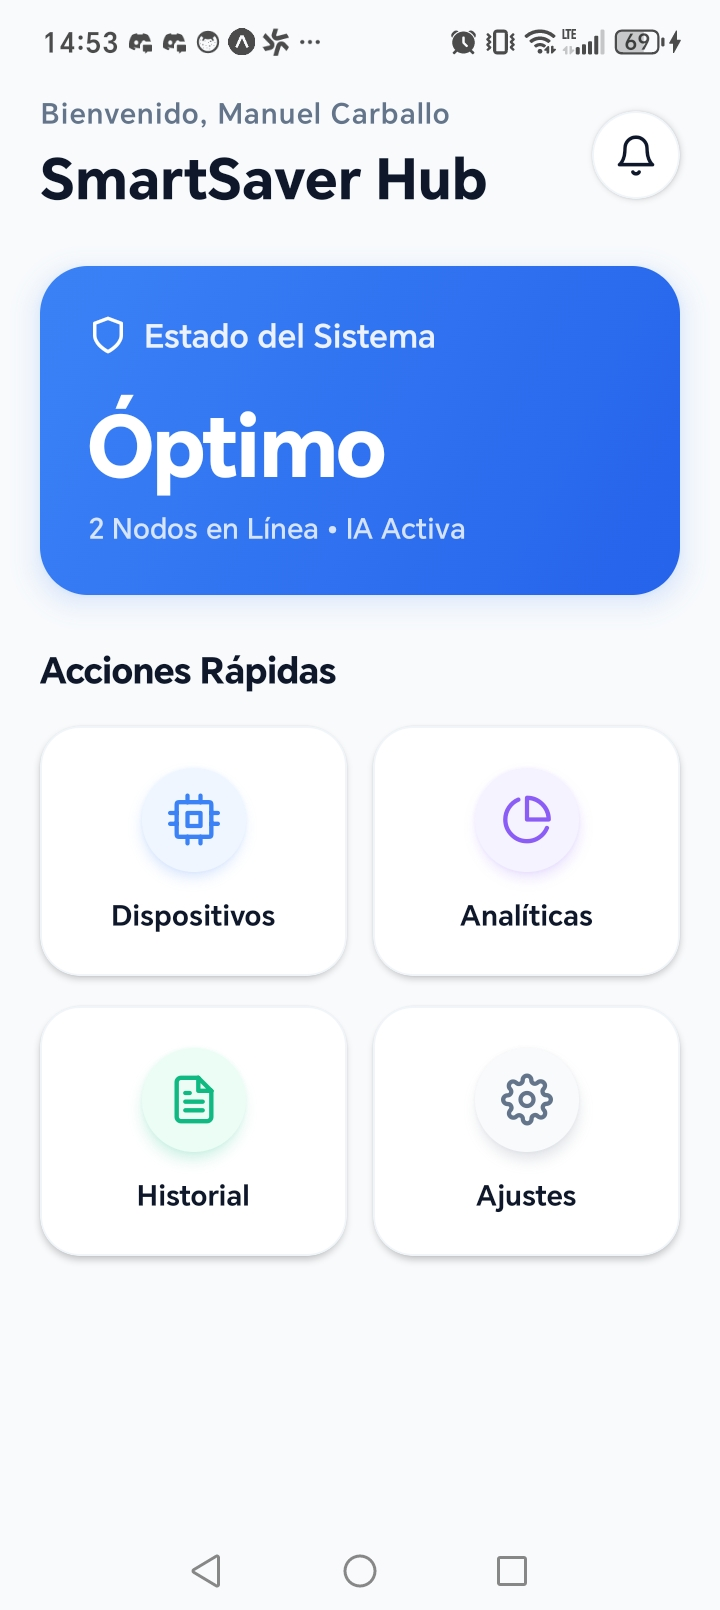
\includegraphics[width=0.45\textwidth]{aplicacion_ss/HOMESCREEN.jpg}
    \caption{Dashboard del Sistema - Panel de Control de Inicio}
    \label{fig:homescreen}
\end{figure}

El panel de inicio o \textbf{Dashboard} es la pantalla de bienvenida y el centro de control principal de la aplicación. Desde esta vista centralizada, el usuario puede acceder a todas las funcionalidades principales del ecosistema SmartSaver a través de accesos directos intuitivos y de rápida navegación.

\subsection{Componentes Clave del Dashboard}
\begin{itemize}
    \item \textbf{Saludo y Encabezado Personalizado:} Muestra un saludo dinámico ("Bienvenido, Usuario") y el título del aplicativo centralizado.
    \item \textbf{Estado del Sistema:} Una tarjeta superior destacada que diagnostica en tiempo real si el estado general de la red es \textit{Óptimo} (si hay nodos inteligentes en línea) o \textit{Crítico} (si todos los nodos se encuentran fuera de línea). También reporta el número exacto de nodos activos en línea y si el motor de Inteligencia Artificial se encuentra activo.
    \item \textbf{Acciones Rápidas (Navegación General):} Cuatro botones interactivos en forma de cuadrícula de alta visibilidad para un acceso inmediato:
    \begin{itemize}
        \item \textbf{Dispositivos:} Dirige a la lista de dispositivos Mini-UPS activos y configuraciones individuales.
        \item \textbf{Analíticas:} Permite visualizar el historial de potencia, gráficos donut y exportación de reportes.
        \item \textbf{Historial:} Da acceso directo a la bitácora local de 200 eventos en tiempo real.
        \item \textbf{Ajustes:} Abre el panel de configuración global del aplicativo, perfil, modo oscuro y conexión del backend.
    \end{itemize}
\end{itemize}

% ==========================================
% SECCIÓN 4: DISPOSITIVOS ACTIVOS
% ==========================================
\section{Dispositivos Activos (Lista de Equipos)}

\begin{figure}[H]
    \centering
    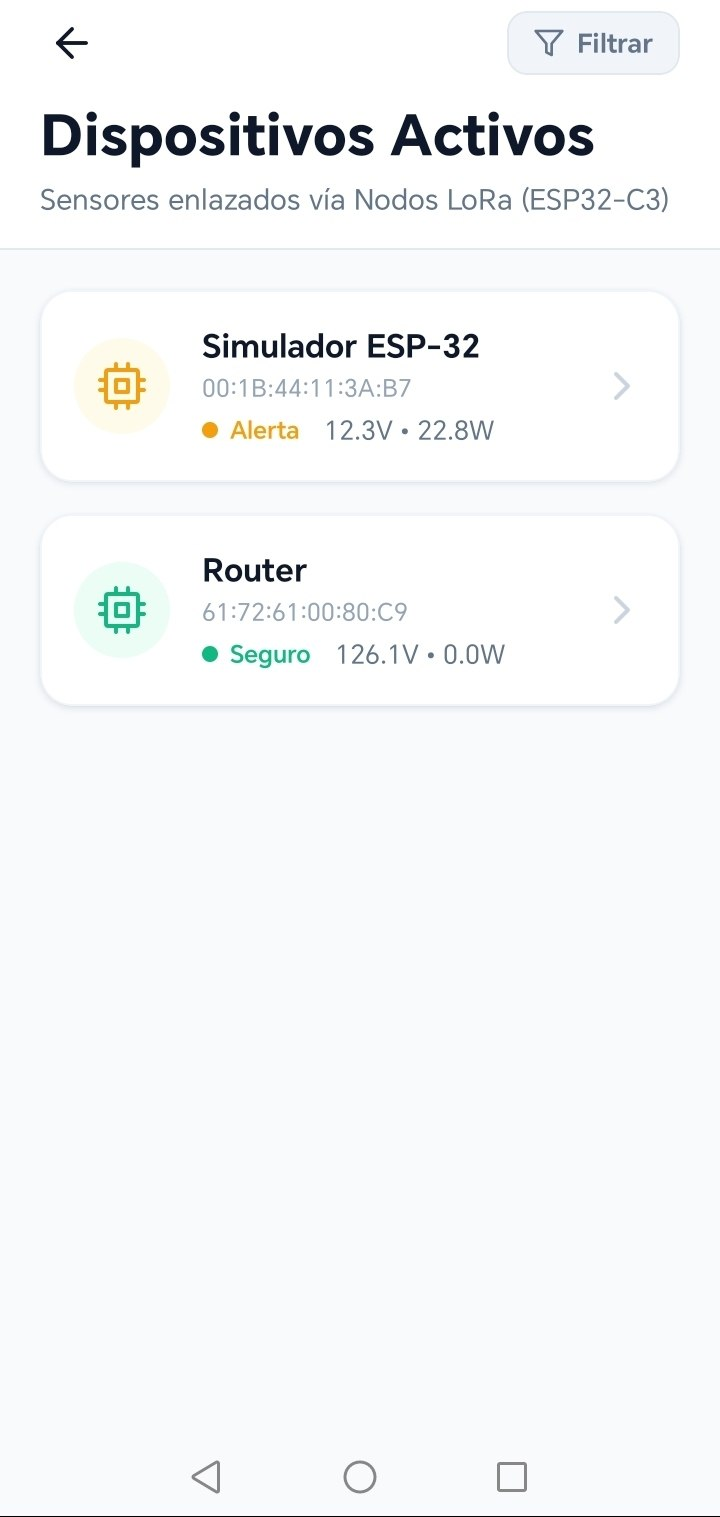
\includegraphics[width=0.45\textwidth]{aplicacion_ss/ACTIVE_DEVICES.jpg}
    \caption{Pantalla de Dispositivos Activos (Lista de Equipos)}
    \label{fig:active_devices}
\end{figure}

La pantalla de \textbf{Dispositivos Activos} se despliega al presionar el botón "Dispositivos" en la sección de Acciones Rápidas del Dashboard, y representa el registro central de todos los equipos Smart Mini-UPS enlazados a su cuenta de usuario.

\subsection{Componentes Visuales de la Lista}
\begin{itemize}
    \item \textbf{Panel de Filtro de Prioridad:} En la parte superior, junto al título de "Dispositivos Activos", se encuentra un botón de "Filtrar" que despliega un panel de filtros interactivos con las opciones \textbf{Todos}, \textbf{P1}, \textbf{P2} y \textbf{P3}. Estos filtros permiten depurar y listar los dispositivos correspondientes a cada nivel de prioridad seleccionado instantáneamente.
    \item \textbf{Tarjetas de Dispositivos:} Cada dispositivo se representa mediante una tarjeta de control que muestra:
    \begin{itemize}
        \item Nombre personalizado del equipo (o dirección MAC en su defecto).
        \item Zona de Seguridad de IA: Diagnóstico en tiempo real basado en la potencia activa (\textit{Seguro} en verde, \textit{Alerta} en naranja o \textit{Crítico} en rojo).
        \item Nivel de prioridad asignado (\textbf{P1}, \textbf{P2} o \textbf{P3}).
        \item Lecturas de Telemetría: Visualización inmediata del voltaje y potencia del nodo (por ejemplo, \textit{12.3V • 22.8W}).
    \end{itemize}
\end{itemize}

\subsection{Registro de Respaldo (Fallback)}
Si por fallas de conexión no se logra establecer contacto inicial con el servidor FastAPI, el aplicativo cargará automáticamente un dispositivo de respaldo configurado en el sistema (\textbf{DEVICE\_REGISTRY}), permitiendo acceder a interfaces de prueba e historial local en memoria.

% ==========================================
% SECCIÓN 5: PANEL DE DETALLE
% ==========================================
\section{Panel de Detalle del Dispositivo}

\begin{figure}[H]
    \centering
    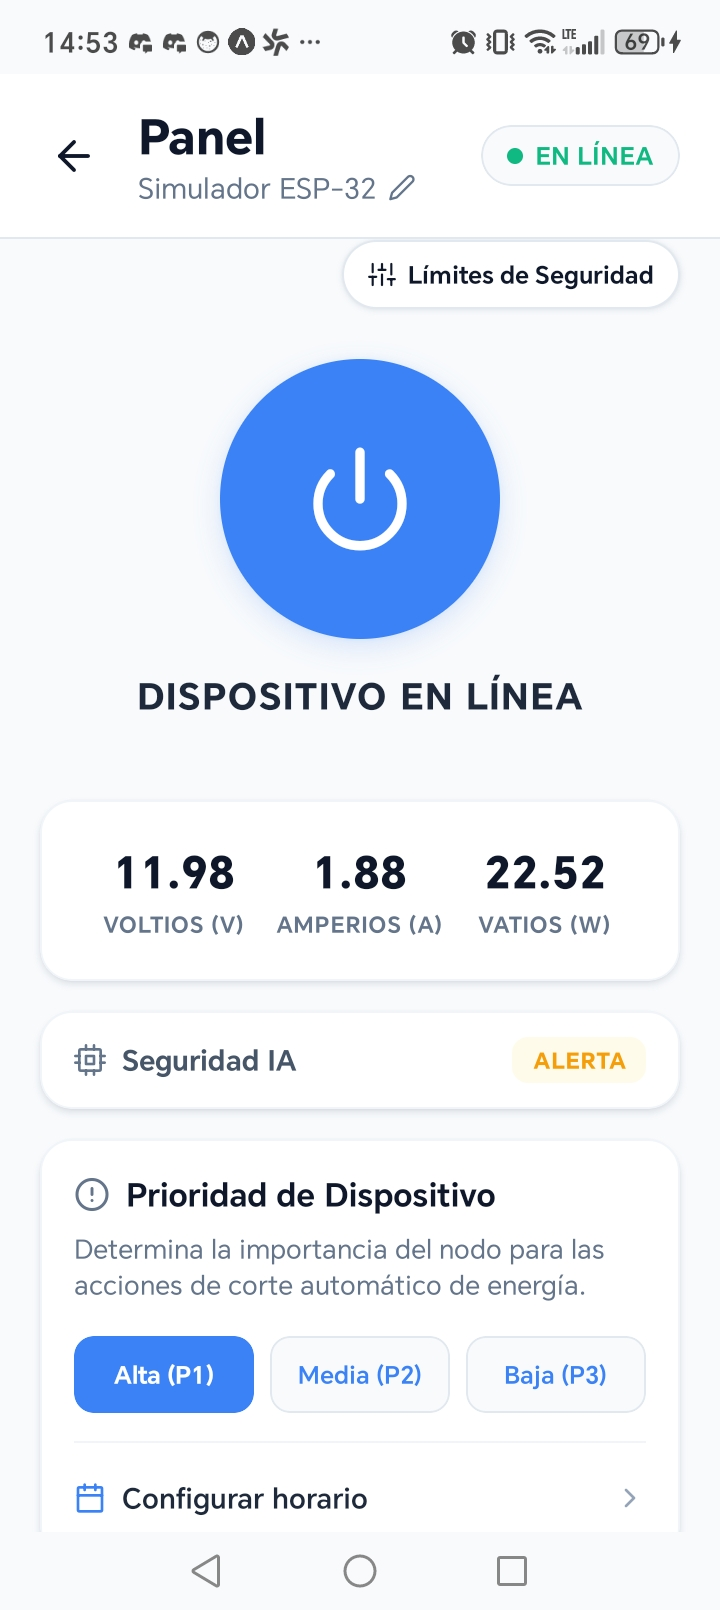
\includegraphics[width=0.45\textwidth]{aplicacion_ss/DEVICE_SCREEN.jpg}
    \caption{Interfaz del Panel de Detalle del Dispositivo Smart Mini-UPS}
    \label{fig:device_screen}
\end{figure}

Al hacer clic sobre cualquier dispositivo de la lista de equipos activos, ingresará al \textbf{Panel de Detalle} (Panel de Control de Relevo), donde se concentra la mayor actividad operativa del sistema.

\subsection{Encabezado Inteligente}
El encabezado del Panel de Detalle provee la información más crítica de un vistazo:
\begin{itemize}
    \item \textbf{Título / Nombre Personalizado:} Visualiza el nombre amigable que le dio a su Mini-UPS. Si hace clic sobre el icono de lápiz a un costado, podrá cambiar o eliminar este nombre personalizado mediante una ventana modal emergente.
    \item \textbf{Píldora de Estado de Red:} Muestra si el equipo está reportando datos de forma activa en los últimos segundos (\textit{En Línea}) o si se ha desconectado de la puerta de enlace (reflejándose como \textit{Off}).
\end{itemize}

\subsection{Interruptor Central de Encendido (Relé)}
En el centro de la pantalla se despliega un gran botón circular interactivo con el símbolo de alimentación:
\begin{itemize}
    \item \textbf{Encendido (Azul brillante):} Indica que el relé físico está transmitiendo corriente de alimentación a los aparatos conectados.
    \item \textbf{Apagado (Gris/Blanco):} El relevador físico está desactivado.
    \item \textbf{Estado de Sincronización (Texto interactivo):} La interfaz refleja de forma continua el estado exacto de la operación: \textbf{DISPOSITIVO INALCANZABLE} (offline), \textbf{SINCRONIZANDO...} (en caso de retraso en confirmación MQTT), \textbf{ENVIANDO COMANDO...} (mientras se transmite la instrucción), \textbf{DISPOSITIVO EN LÍNEA} (activo) o \textbf{DISPOSITIVO DESCONECTADO} (inactivo).
\end{itemize}

\begin{alertBox}
Si un dispositivo se encuentra en estado fuera de línea, el botón central se deshabilitará automáticamente en color gris plano y se mostrará un banner rojo de advertencia superior. No intente enviar comandos MQTT hasta restaurar la conexión de red del equipo.
\end{alertBox}

\subsection{Evaluación de Seguridad por IA Integrada}
El Panel de Detalle incluye una sección dedicada a la \textbf{Seguridad IA}. Esta tarjeta indica en tiempo real la clasificación de riesgo energético del dispositivo con estados correspondientes como \textbf{SEGURO} (verde), \textbf{ALERTA} (naranja) o \textbf{CRÍTICO} (rojo). Si el dispositivo no tiene señal o está apagado, se reflejará como \textbf{SIN SEÑAL} o \textbf{EN ESPERA}.

\subsection{Visualización de Telemetría}
Bajo el control central, una tarjeta dividida en tres columnas le muestra de forma precisa el consumo eléctrico instantáneo:
\begin{enumerate}
    \item \textbf{Voltios (V):} Tensión entregada por la batería/red eléctrica.
    \item \textbf{Amperios (A):} Corriente consumida por la carga conectada.
    \item \textbf{Vatios (W):} Potencia activa total consumida en tiempo real (Calculada como $P = V \times I$).
\end{enumerate}

% ==========================================
% SECCIÓN 6: INTELIGENCIA ARTIFICIAL
% ==========================================
\section{Evaluación de Seguridad por Inteligencia Artificial}

\begin{table}[htbp]
    \centering
    \caption{Zonas de Diagnóstico de Energía IA}
    \begin{tabular}{lccl}
        \toprule
        \textbf{Zona de Seguridad} & \textbf{Rango (W)} & \textbf{Color de Marca} & \textbf{Acción del Sistema} \\
        \midrule
        \textbf{SEGURO} & 0.0W - 15.0W & Verde (\#10B981) & Funcionamiento normal garantizado. \\
        \textbf{ALERTA} & 15.1W - 30.0W & Naranja (\#F59E0B) & Alerta preventiva por alto consumo. \\
        \textbf{CRÍTICO} & $>$ 30.0W & Rojo (\#EF4444) & Advertencia crítica de sobrecarga en Mini-UPS. \\
        \bottomrule
    \end{tabular}
\end{table}

La aplicación cuenta con un motor de diagnóstico inteligente que analiza la potencia instantánea y clasifica el riesgo operativo del Mini-UPS en tres zonas distintas de seguridad, generando alertas automáticas basadas en la potencia en vatios.

\subsection{Notificaciones y Registro de Transición de Zona}
Cuando el equipo transita de una zona a otra, el sistema móvil ejecuta tres tareas:
\begin{enumerate}
    \item Actualiza el color de la tarjeta de "Seguridad IA" del panel.
    \item Registra una entrada formal en el \textbf{Historial de Eventos} con severidad preventiva (\textit{Warning}) o grave (\textit{Critical}).
    \item Dispara una notificación nativa en la barra superior de su terminal móvil para alertarlo de inmediato sobre la fluctuación de carga de energía.
\end{enumerate}

% ==========================================
% SECCIÓN 7: LÍMITES DE SEGURIDAD
% ==========================================
\section{Configuración de Umbrales y Límites de Seguridad}

\begin{figure}[H]
    \centering
    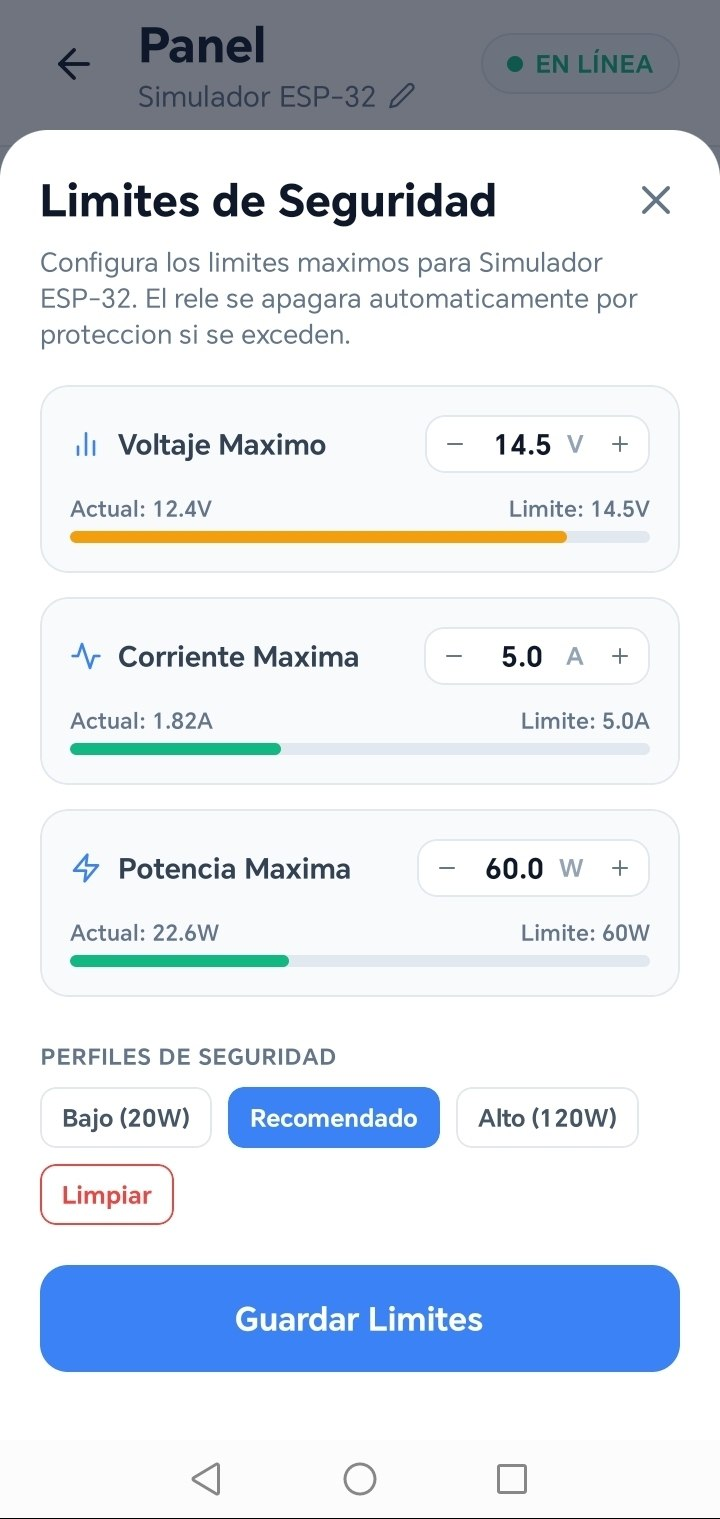
\includegraphics[width=0.45\textwidth]{aplicacion_ss/ENERGY_LIMITS_SETUP.jpg}
    \caption{Configuración de Límites Eléctricos de Seguridad}
    \label{fig:energy_limits_setup}
\end{figure}

Para evitar fallas catastróficas o sobrecalentamiento, SmartSaver le permite establecer límites máximos de tolerancia eléctrica. Si el dispositivo supera cualquiera de estos valores, se ejecutará un \textbf{Apagado de Emergencia automático} por seguridad.

\subsection{Acceso e Interfaz de Límites}
En la zona superior del Scroll, justo abajo del encabezado principal a la derecha, encontrará un botón destacado con la leyenda \textbf{"Límites de Seguridad"}. Al presionarlo, se deslizará la hoja de configuración de umbrales.

\subsection{Ajustes Eléctricos Disponibles}
Para cada métrica crítica, podrá configurar umbrales exactos:
\begin{itemize}
    \item \textbf{Voltaje Máximo (Límite: $0.1V - 60.0V$):} Evita fluctuaciones dañinas de voltaje.
    \item \textbf{Corriente Máxima (Límite: $0.1A - 30.0A$):} Evita cortocircuitos o demandas extremas de amperaje.
    \item \textbf{Potencia Máxima (Límite: $0.1W - 500.0W$):} Máxima capacidad de carga permitida en vatios.
\end{itemize}

\subsection{Métodos de Entrada Intuitivos y Premium}
Para máxima comodidad, el aplicativo móvil ofrece tres formas de entrada de datos interactivos:
\begin{enumerate}
    \item \textbf{Controles Incrementales (Steppers):} Teniendo botones \textbf{[-]} y \textbf{[+]} a cada lado del indicador para realizar micro-ajustes rápidos:
    \begin{itemize}
        \item \textbf{Voltaje:} Incrementos/decrementos de $\pm 0.5V$.
        \item \textbf{Corriente:} Incrementos/decrementos de $\pm 0.1A$.
        \item \textbf{Potencia:} Incrementos/decrementos de $\pm 5W$.
    \end{itemize}
    \item \textbf{Ventana Modal de Teclado Numérico (Evita Bloqueo de Pantalla):} Si presiona directamente sobre la cifra de valor numérico del límite, se abrirá un panel de edición flotante \textbf{en el centro exacto de la pantalla}. Esto evita que el teclado del móvil tape la visualización. Ingrese la cantidad deseada mediante el teclado numérico interactivo y presione \textbf{"Confirmar"} para guardarlo de manera segura.
    \item \textbf{Perfiles Rápidos de Seguridad (Presets):} En la base de la ventana, puede seleccionar perfiles rápidos optimizados:
    \begin{itemize}
        \item \textbf{Bajo (20W):} Configura voltaje a $12V$, corriente a $2A$ y potencia a $20W$.
        \item \textbf{Recomendado:} Configura voltaje a $14.5V$, corriente a $5A$ y potencia a $60W$.
        \item \textbf{Alto (120W):} Configura voltaje a $28V$, corriente a $10A$ y potencia a $120W$.
        \item \textbf{Limpiar:} Remueve todos los límites de seguridad activos del dispositivo.
    \end{itemize}
\end{enumerate}

\begin{infoBox}
Cuando los límites configurados en el panel móvil coincidan exactamente con uno de los perfiles rápidos (\textit{Bajo}, \textit{Recomendado} o \textit{Alto}), la píldora correspondiente se iluminará en color \textbf{azul sólido} (\#3B82F6), dándole confirmación visual inmediata del perfil activo.
\end{infoBox}

\subsection{Medidores Visuales Comparativos en Tiempo Real}
Cada tarjeta de límite posee un medidor de barra de progreso que compara la \textbf{telemetría viva actual} con el \textbf{umbral programado}. La barra cambia de color según el nivel de carga actual:
\begin{itemize}
    \item \textbf{Verde (Consumo Normal):} Inferior al 75\% del límite configurado.
    \item \textbf{Naranja (Zona de Advertencia):} Entre el 75\% y el 90\% del límite configurado.
    \item \textbf{Rojo (Nivel Crítico de Desconexión):} Excede el 90\% del límite configurado.
\end{itemize}

\subsection{Guardado Seguro de Parámetros}
Una vez establecidos los umbrales correspondientes mediante cualquiera de los métodos indicados, presione el botón destacado \textbf{"Guardar Limites"} ubicado en la base de la interfaz para persistir y transferir estos parámetros al firmware del ESP32 a través de la pasarela de control.

% ==========================================
% SECCIÓN 8: PRIORIDADES Y HORARIOS
% ==========================================
\section{Niveles de Prioridad y Configuración de Horarios}

\begin{figure}[H]
    \centering
    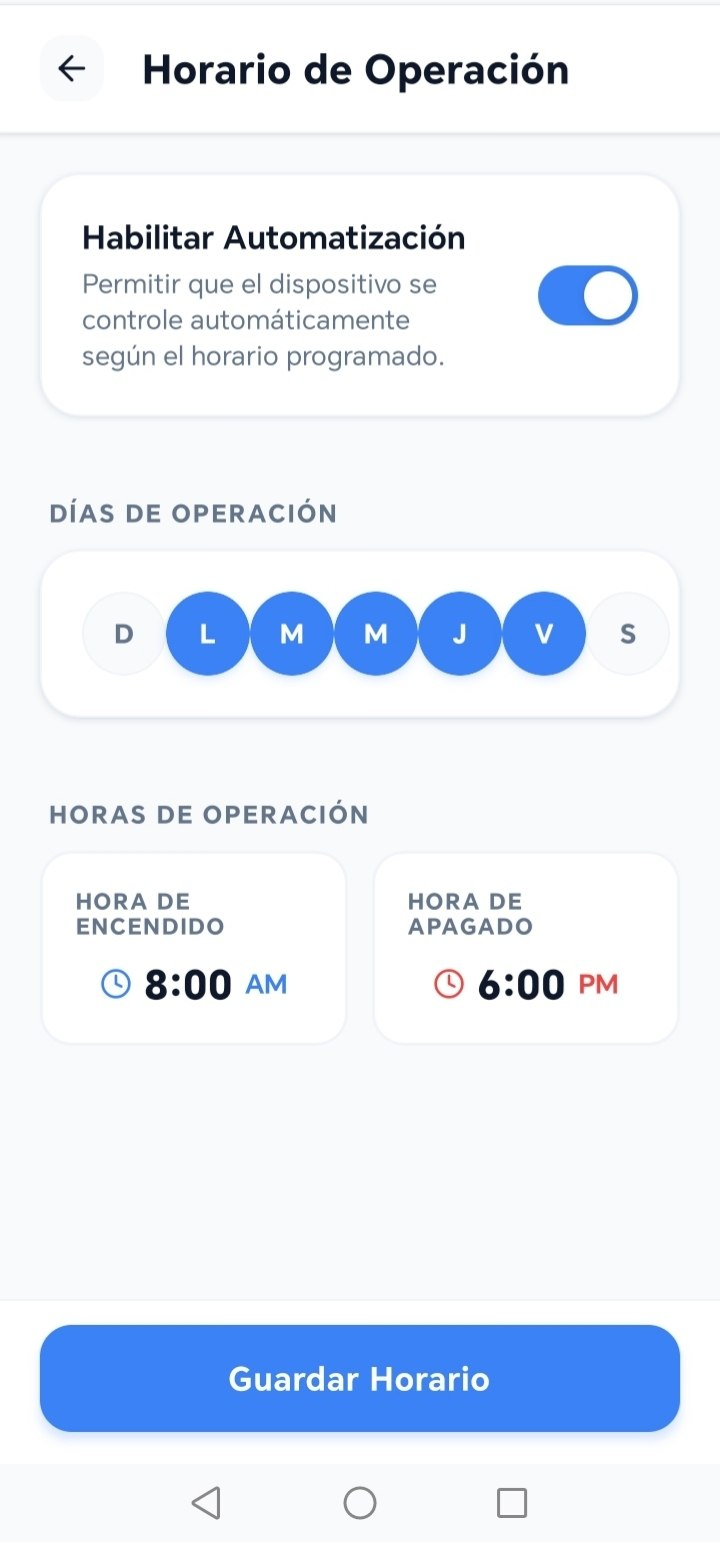
\includegraphics[width=0.45\textwidth]{aplicacion_ss/ScheduleScreen.jpg}
    \caption{Configuración de Horarios y Automatización de Encendido/Apagado}
    \label{fig:schedule_screen}
\end{figure}

El sistema permite automatizar las operaciones diarias y la jerarquía de corte inteligente para asegurar que los recursos de red más críticos no sufran cortes accidentales.

\subsection{Prioridad del Dispositivo (Corte Inteligente)}
En la tarjeta de "Prioridad de Dispositivo", configure la jerarquía del equipo para la toma de decisiones del algoritmo del backend:
\begin{itemize}
    \item \textbf{Alta (P1):} Dispositivos sumamente críticos (por ejemplo, enrutadores de red principales o servidores locales). Son los últimos en desconectarse en caso de emergencia de energía en la red de baterías.
    \item \textbf{Media (P2):} Configuración predeterminada y estándar del sistema.
    \item \textbf{Baja (P3):} Dispositivos secundarios de baja prioridad. Serán apagados de forma prioritaria en caso de registrarse niveles deficientes de energía global.
\end{itemize}

\subsection{Configuración de Horarios de Operación y Automatización}
Al presionar la opción \textbf{"Configurar horario"} en el Panel de Detalle, se ingresa a la pantalla de \textbf{Horario de Operación} (Figura~\ref{fig:schedule_screen}), la cual permite parametrizar las franjas de funcionamiento automatizado.

\begin{itemize}
    \item \textbf{Habilitar Automatización:} Un interruptor principal permite activar o desactivar el control horario automático. Al desactivarse, el resto de configuraciones de la interfaz se atenuará y deshabilitará.
    \item \textbf{Días de Operación:} Selector intuitivo mediante botones circulares para elegir individualmente los días de la semana (\textbf{Dom, Lun, Mar, Mié, Jue, Vie, Sáb}) en los que aplicará la programación.
    \item \textbf{Horas de Operación:} Tarjetas para definir con precisión la \textbf{Hora de Encendido} (por ejemplo, \textit{8:00 AM}) y la \textbf{Hora de Apagado} (por ejemplo, \textit{6:00 PM}). Al tocarlas se abre un selector de hora modular con rejilla de 12 horas y selector de período AM/PM.
    \item \textbf{Guardar Horario:} Botón final para almacenar localmente y aplicar las directrices del cronograma.
\end{itemize}

% ==========================================
% SECCIÓN 9: HISTORIAL DE EVENTOS
% ==========================================
\section{Historial y Bitácora de Eventos}

\begin{figure}[H]
    \centering
    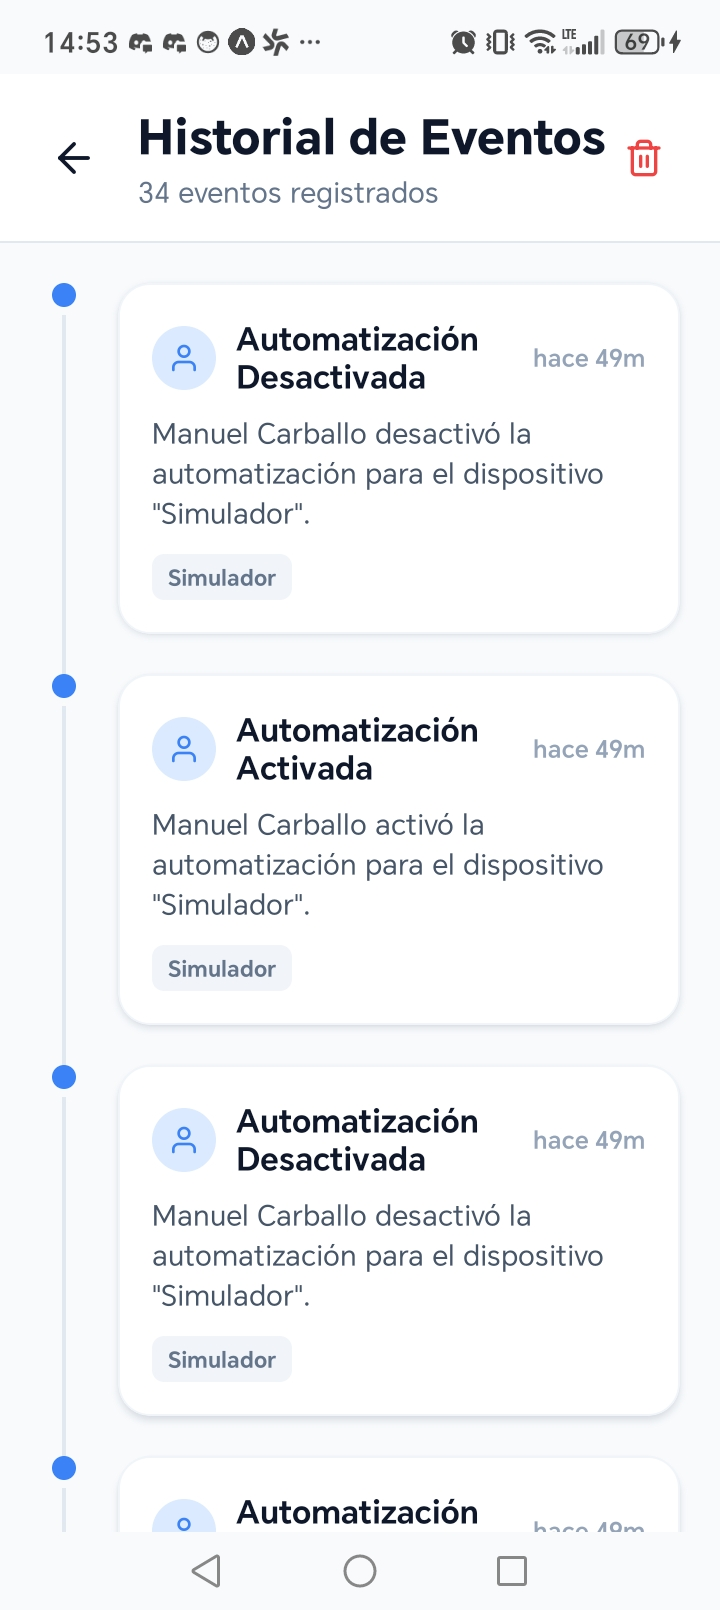
\includegraphics[width=0.45\textwidth]{aplicacion_ss/Events_screen.jpg}
    \caption{Historial y Bitácora de Eventos del Sistema}
    \label{fig:events_screen}
\end{figure}

El sistema guarda localmente mediante almacenamiento persistente indexado (\textit{AsyncStorage}) una bitácora detallada con los últimos \textbf{200 eventos} de su ecosistema:
\begin{itemize}
    \item \textbf{USER\_ACTION:} Registro de comandos de encendido/apagado remotos, cambios de prioridad de red, o modificación de umbrales eléctricos por el usuario.
    \item \textbf{SYSTEM / AI\_ACTION:} Reconexión de red de dispositivos, normalización de carga eléctrica, restauraciones del sistema.
    \item \textbf{WARNING:} Transiciones a zonas de alerta eléctrica y detecciones preventivas por alto consumo de vatios.
    \item \textbf{CRITICAL (Corte por Límite Excedido):} Alertas críticas, caídas del enlace de red físicas y, sobre todo, \textbf{eventos de apagado de emergencia} preventivos cuando se sobrepasa algún límite de voltaje, corriente o potencia configurado.
\end{itemize}

\subsection{Funcionalidades de la Interfaz de Historial}
\begin{itemize}
    \item \textbf{Botón de Limpieza (Papelera):} En la esquina superior derecha del encabezado, un botón rojo de papelera permite eliminar por completo la bitácora local almacenada mediante una confirmación de seguridad.
    \item \textbf{Estructura de la Bitácora:} Cada evento se despliega en una tarjeta con una línea de tiempo coloreada por severidad, indicando el tipo de acción, una descripción clara y una etiqueta o píldora con el nombre del nodo asociado (por ejemplo, \textit{"Simulador"}).
\end{itemize}

% ==========================================
% SECCIÓN 10: ANALÍTICAS Y EXPORTACIÓN
% ==========================================
\section{Módulo de Analíticas e Históricos Avanzados}

\begin{figure}[H]
    \centering
    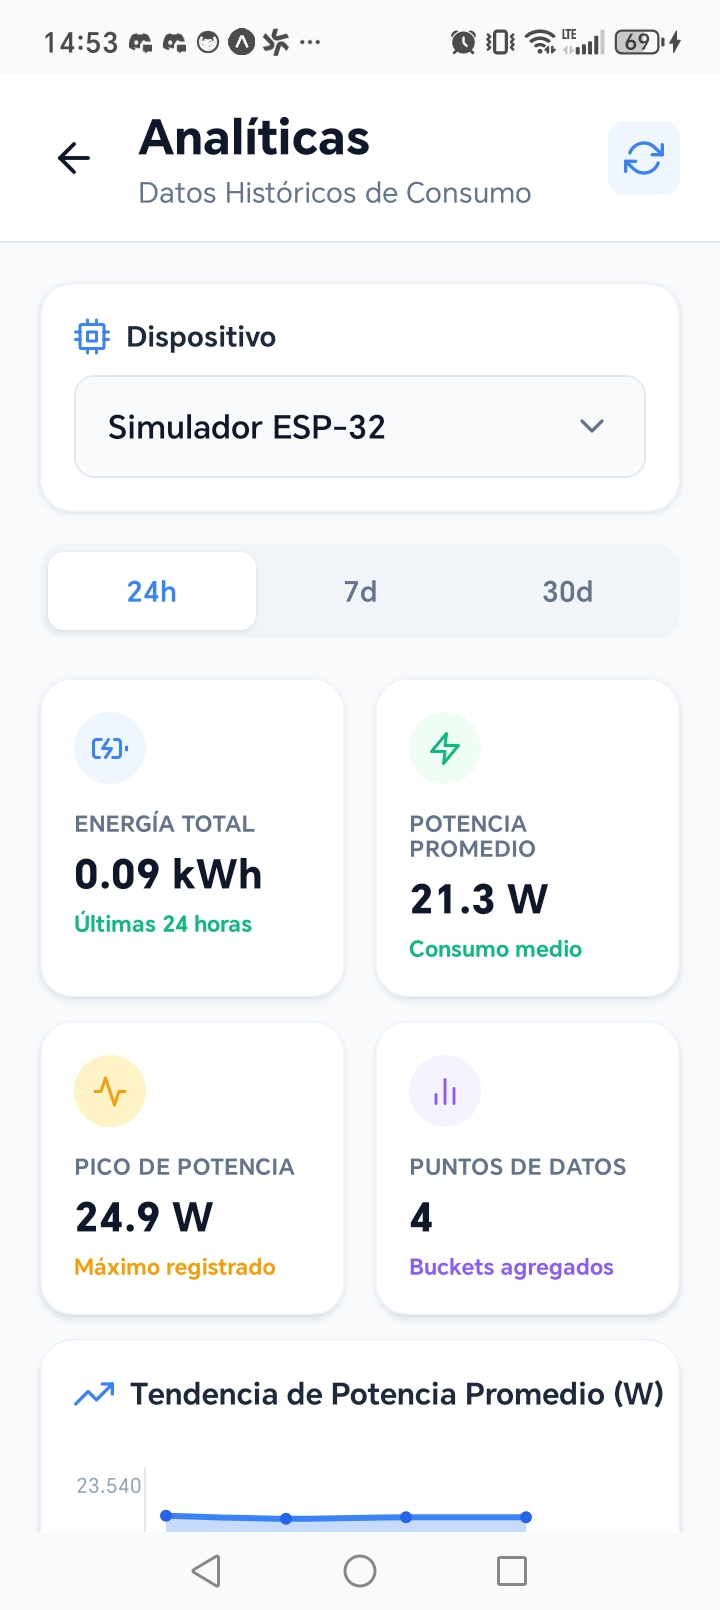
\includegraphics[width=0.45\textwidth]{aplicacion_ss/ANALYTICS_1.jpg}
    \caption{Pantalla de Analíticas: Resumen de Consumo Eléctrico}
    \label{fig:analytics_1}
\end{figure}

\subsection{Selector de Rango de Tiempo y Granularidad}
Puede auditar datos cambiando filtros interactivos:
\begin{itemize}
    \item \textbf{Filtros de Periodo:} Visualice las últimas \textbf{24 horas}, \textbf{7 días} o \textbf{30 días}.
    \item \textbf{Dispositivo Activo:} Seleccione cualquier Mini-UPS de la lista para analizar su historial.
\end{itemize}

\subsection{Tarjetas Resumen de Consumo}
En la parte superior de la pantalla, se despliegan cuatro tarjetas resumen diseñadas para proporcionar un diagnóstico instantáneo de la telemetría acumulada:
\begin{itemize}
    \item \textbf{Energía Total:} Consumo total de energía durante el período seleccionado expresado en Kilovatios-hora (kWh).
    \item \textbf{Potencia Promedio:} El nivel de potencia medio (W) en el período actual.
    \item \textbf{Pico de Potencia:} El valor máximo registrado de vatios de consumo (W).
    \item \textbf{Puntos de Datos:} La cantidad total de registros de telemetría o buckets agregados analizados.
\end{itemize}
Adicionalmente, se cuenta con un botón de refresco (\textit{refresh-cw}) en la esquina superior derecha para recargar inmediatamente los datos históricos desde la base de datos FastAPI.

\subsection{Visualización Gráfica}

\begin{figure}[H]
    \centering
    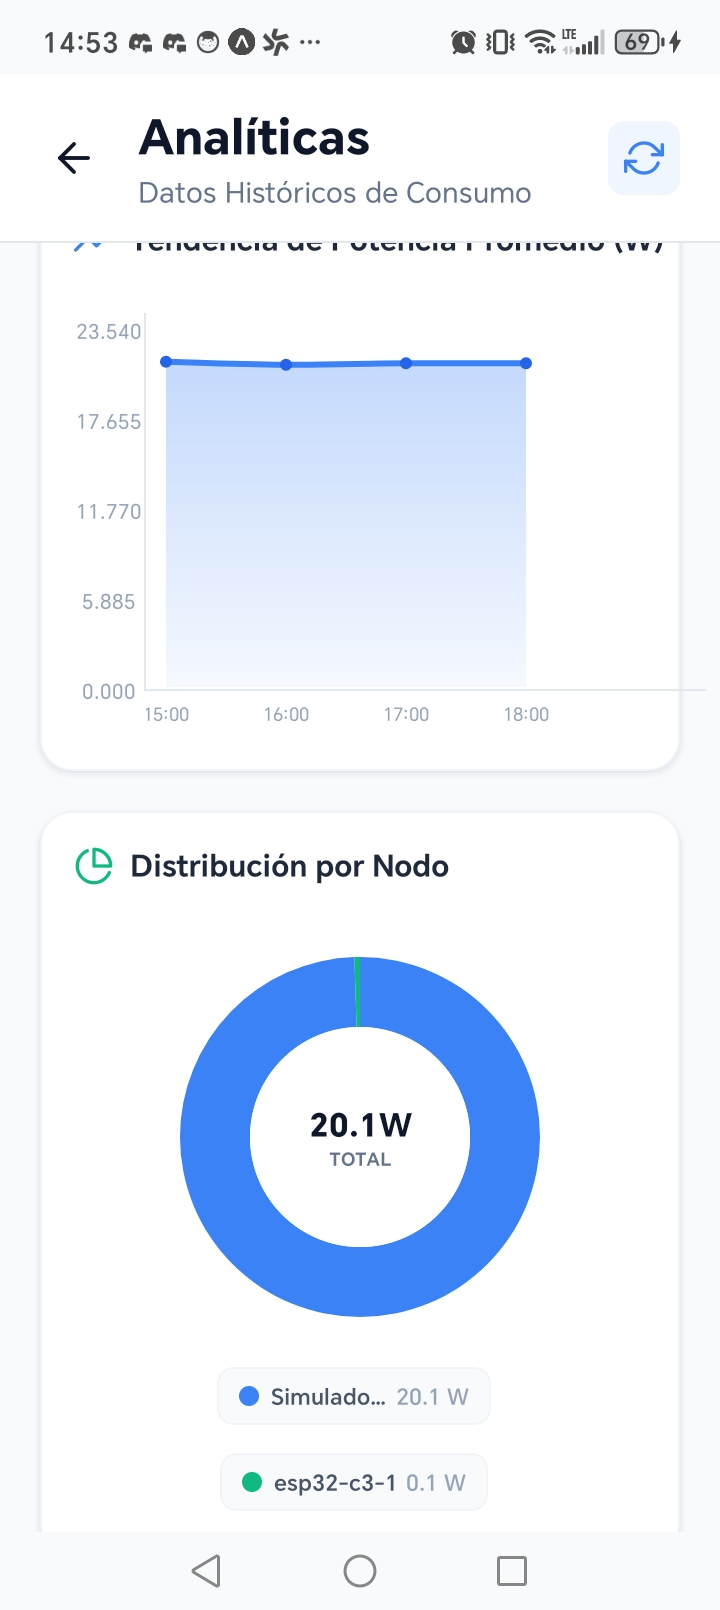
\includegraphics[width=0.45\textwidth]{aplicacion_ss/ANALYTICS_2.jpg}
    \caption{Visualización Gráfica: Distribución por Nodo e Historial de Potencia}
    \label{fig:analytics_2}
\end{figure}

\begin{enumerate}
    \item \textbf{Tendencia de Potencia Promedio (W):} Gráfico lineal sombreado de alta densidad y suave curvatura que ayuda a diagnosticar de manera continua los picos y valles de vatios de consumo del dispositivo activo.
    \item \textbf{Distribución por Nodo (Gráfico Donut):} Un moderno e interactivo gráfico circular tipo donut que representa proporcionalmente qué porcentaje del consumo total corresponde a cada equipo. En el centro de la dona se refleja la cifra de potencia total global consumida.
    \item \textbf{Energía por Periodo (Wh):} Un gráfico lineal que ilustra de manera detallada la acumulación de vatios-hora a lo largo de las divisiones de tiempo seleccionadas.
\end{enumerate}

\subsection{Exportación de Reportes}

\begin{figure}[H]
    \centering
    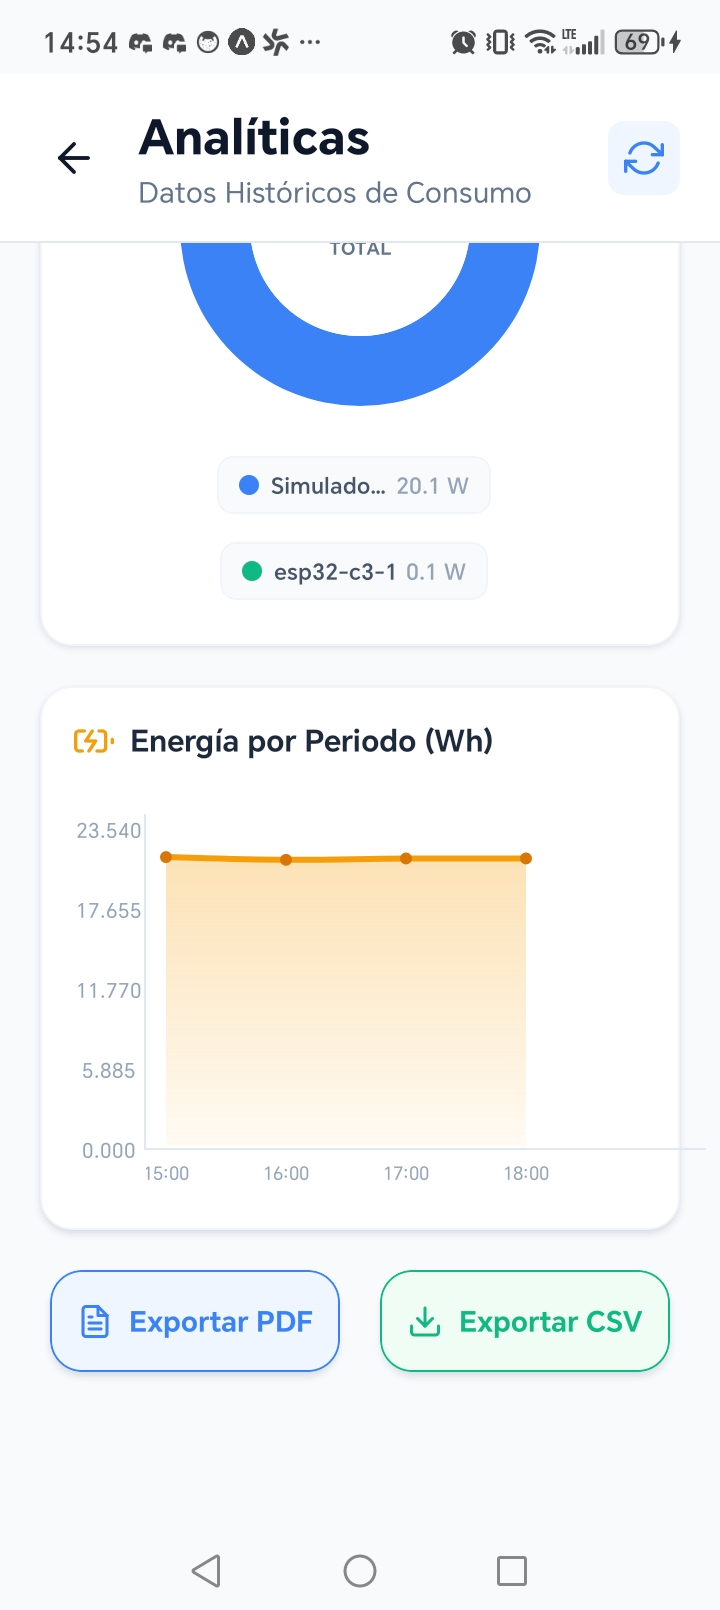
\includegraphics[width=0.45\textwidth]{aplicacion_ss/ANALYTICS_3.jpg}
    \caption{Exportación de Reportes e Históricos de Energía}
    \label{fig:analytics_3}
\end{figure}

Utilice los botones en la parte inferior para descargar y compartir sus datos:
\begin{itemize}
    \item \textbf{Exportar a CSV:} Genera un reporte detallado delimitado por comas de toda la telemetría recolectada en el periodo de tiempo configurado.
    \item \textbf{Exportar a PDF:} Crea un reporte visual estructurado, óptimo para la impresión física o presentación formal de auditoría de energía.
\end{itemize}

% ==========================================
% SECCIÓN 11: CONFIGURACIÓN GLOBAL
% ==========================================
\section{Configuración Global y Ajustes de la Aplicación}

\begin{figure}[H]
    \centering
    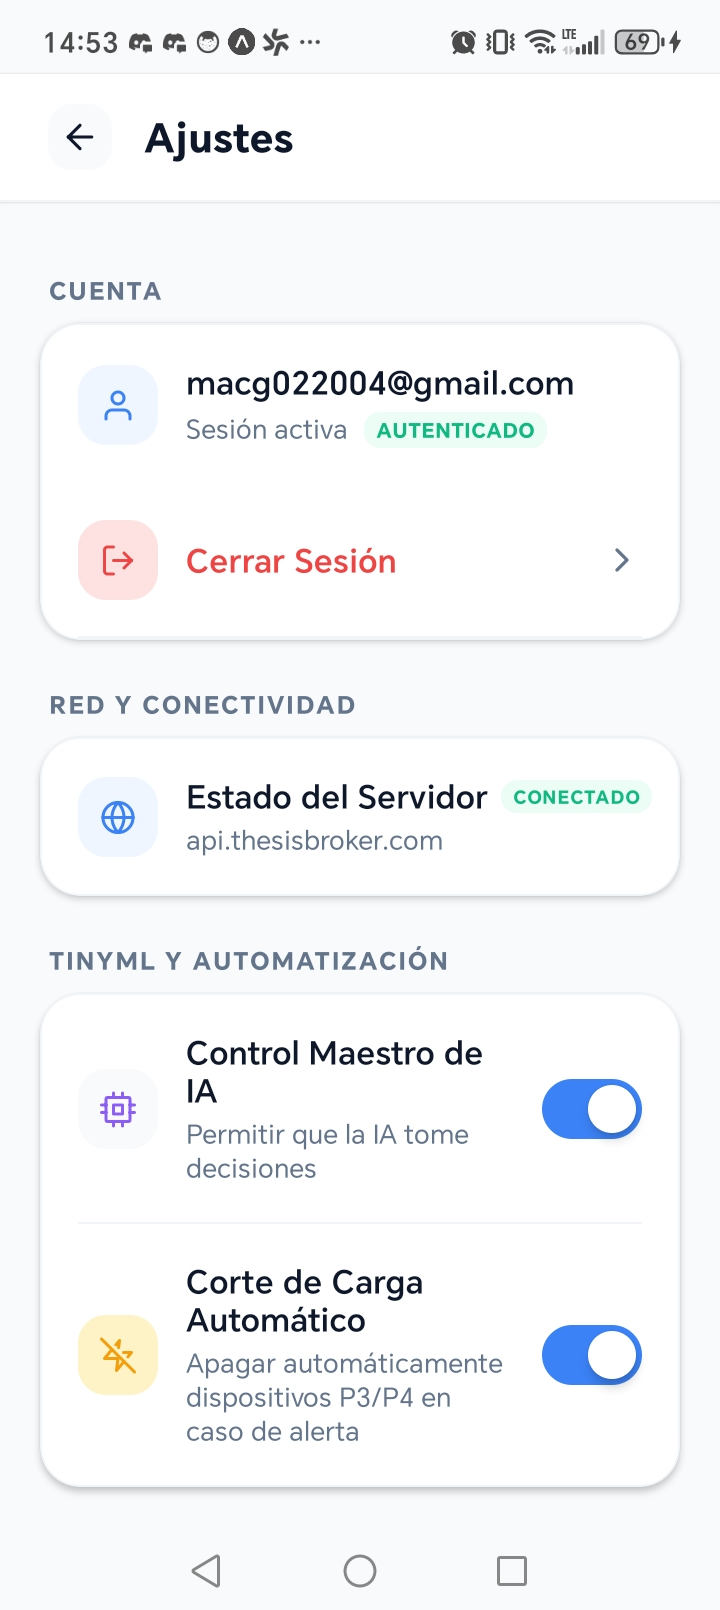
\includegraphics[width=0.45\textwidth]{aplicacion_ss/SETTINGS_SCREEN_1.jpg}
    \caption{Pantalla de Ajustes del Sistema - Configuración Global}
    \label{fig:settings_screen_1}
\end{figure}

\begin{figure}[H]
    \centering
    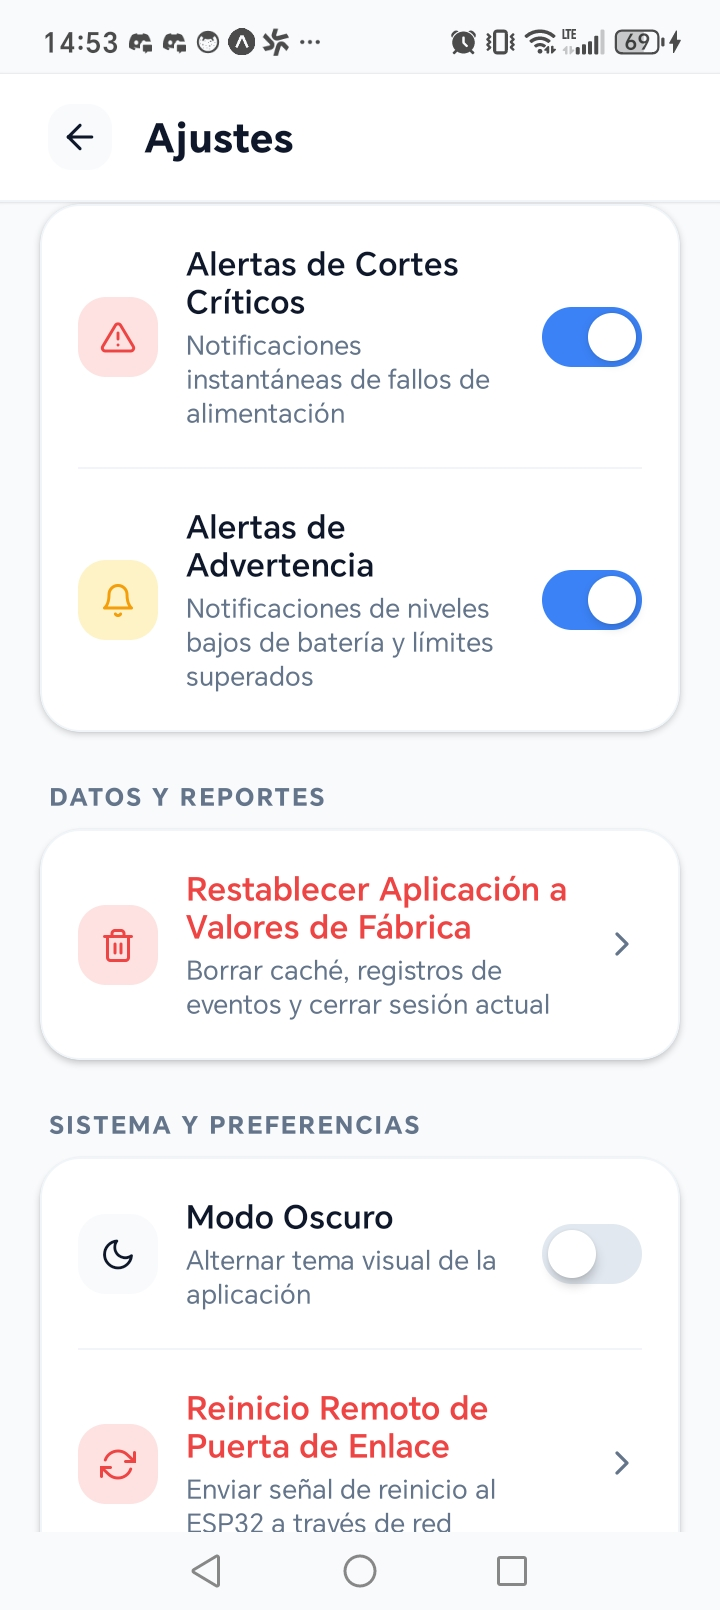
\includegraphics[width=0.45\textwidth]{aplicacion_ss/SETTINGS_SCREEN_2.jpg}
    \caption{Pantalla de Ajustes del Sistema - Notificaciones, Preferencias y Control de Puerta de Enlace}
    \label{fig:settings_screen_2}
\end{figure}

El módulo de \textbf{Ajustes} proporciona acceso a preferencias del terminal, seguridad del usuario, conectividad del servidor backend, control inteligente y borrado preventivo de datos.

\subsection{Opciones de Configuración Disponibles}
\begin{itemize}
    \item \textbf{Gestión de Cuenta:} Muestra información detallada sobre la sesión de usuario activa autenticada a través de Auth0 (PKCE) y un botón interactivo para el cierre seguro de sesión.
    \item \textbf{Conectividad de Red:} Muestra el estado del servidor backend en tiempo real (Conectado/Desconectado) junto a la dirección base de la pasarela API REST/WebSocket centralizada.
    \item \textbf{Control Maestro de IA:} Un interruptor maestro que habilita o inhabilita el motor inteligente de toma de decisiones del servidor. Al apagarlo, la IA no enviará alertas automatizadas por fluctuación o cortes de emergencia.
    \item \textbf{Corte de Carga Automático:} Permite que el sistema apague automáticamente los dispositivos de baja prioridad (P3/P4) en caso de que se detecte una alerta en el consumo de energía general de la red. Este toggle está vinculado e integrado con el Control Maestro de IA.
    \item \textbf{Alertas y Notificaciones:} Permite activar o desactivar notificaciones del sistema de manera segmentada para \textbf{Cortes Críticos} y \textbf{Mensajes de Advertencia} (Figura~\ref{fig:settings_screen_2}).
    \item \textbf{Preferencias del Sistema (Modo Oscuro):} Interruptor interactivo para cambiar de manera instantánea entre el tema de modo claro y el modo oscuro con persistencia de preferencias.
    \item \textbf{Reinicio Remoto de Puerta de Enlace:} Botón interactivo que permite enviar una señal remota vía red para reiniciar de manera forzada el hardware de la Puerta de Enlace ESP32.
    \item \textbf{Datos y Reportes (Restablecer Fábrica):} Botón destacado en color rojo para depurar por completo la memoria caché local, los históricos locales de eventos en AsyncStorage y desvincular el perfil de red de forma segura.
\end{itemize}

% ==========================================
% SECCIÓN 12: SOLUCIÓN DE PROBLEMAS
% ==========================================
\section{Resolución de Problemas Frecuentes (Troubleshooting)}

\subsection{El botón de encendido no reacciona}
\textbf{Causa:} El dispositivo está en estado \textbf{"Fuera de Línea"}. \\
\textbf{Solución:} Verifique que su ESP32 Mini-UPS se encuentre conectado al router WiFi local y que el backend de FastAPI esté en ejecución. La telemetría debe parpadear en verde en el listado para poder operar comandos remotos.

\subsection{Al cambiar los límites de seguridad manuales no se guardan}
\textbf{Causa:} Ha ingresado un valor fuera del rango límite permitido de bounds. \\
\textbf{Solución:} Al presionar el valor e ingresar datos en el popup centrado, asegúrese de respetar los rangos estrictos: Voltaje ($0.1V - 60.0V$), Corriente ($0.1A - 30.0A$), y Potencia ($0.1W - 500.0W$). Valores inválidos o vacíos no serán confirmados.

\subsection{El gráfico circular no carga datos}
\textbf{Causa:} El servidor backend reporta historial nulo de telemetrías para otros dispositivos en la red. \\
\textbf{Solución:} Mantenga encendidos los demás nodos inteligentes al menos un par de minutos para que sus reportes iniciales se consoliden en la base de datos centralizada MariaDB y el gráfico pueda armar la distribución proporcional.

\end{document}
